%==============================================================================
% ULAL - Unified Lifelong Action Learning (IEEEtran conference, two-column)
% Compile:  pdflatex ulal_paper.tex   (run twice for refs)
% All figures are TikZ schematics drawn in this file (no image files needed).
%==============================================================================
\documentclass[conference]{IEEEtran}

\usepackage[T1]{fontenc}
\usepackage{booktabs}
\usepackage{amsmath}
\usepackage{amssymb}
\usepackage{xcolor}
\usepackage{array}
\usepackage[hidelinks]{hyperref}
\usepackage{tikz}
\usetikzlibrary{arrows.meta,positioning,calc,shapes.geometric,shapes.multipart,shadows}

% ---- one visual language for every schematic in the paper ----
\tikzset{
  ulal/.style={x=1mm, y=1mm, font=\scriptsize},
  u box/.style={draw, rounded corners=2pt, align=center, minimum height=7mm, inner sep=1.2mm},
  u data/.style={u box, fill=gray!12},
  u clip/.style={u box, fill=gray!12, minimum width=9mm,
                 double copy shadow={shadow xshift=0.7mm, shadow yshift=0.7mm}},
  u net/.style={u box, fill=blue!8, minimum width=17mm},
  u frz/.style={u box, fill=white, densely dashed, minimum width=17mm},
  u head/.style={u box, fill=green!16, minimum width=11mm},
  u meta/.style={u box, fill=violet!12},
  u buf/.style={draw, cylinder, shape border rotate=90, aspect=0.25, fill=orange!25,
                minimum height=7mm, minimum width=9mm, align=center, inner sep=0.3mm},
  u op/.style={draw, circle, inner sep=0.4pt, minimum size=5mm, fill=white, font=\tiny},
  u loss/.style={draw, rounded corners=3pt, fill=red!7, inner sep=1mm, font=\tiny, align=center,
                 minimum height=5mm},
  u arr/.style={-{Latex[length=1.7mm]}},
  u dim/.style={font=\tiny, text=black!50, midway, above=-0.3mm},
  u small/.style={font=\tiny, text=black!55},
  u panel/.style={draw=black!20, fill=black!2.5, rounded corners=3pt},
  u best/.style={draw=green!55!black, line width=0.9pt, fill=green!4, rounded corners=3pt},
  u stage/.style={font=\footnotesize\bfseries, anchor=east, align=right},
  u hand/.style={-{Latex[length=2mm]}, thick, black!40},
  u handlab/.style={font=\tiny\itshape, text=black!55, anchor=west},
  u res/.style={font=\footnotesize\bfseries, text=black!75, anchor=east},
  u pick/.style={font=\tiny\bfseries, text=green!45!black, anchor=east},
}
% a split head: old rows | new rows
\newcommand{\headsplit}[4]{%
  \node[draw, rectangle split, rectangle split horizontal, rectangle split parts=2,
        rectangle split part fill={green!26,green!9}, rounded corners=2pt, minimum height=7mm,
        font=\tiny] (#1) at (#2) {#3\nodepart{two}#4};}

\begin{document}

\title{Unified Lifelong Action Learning:\\
A Real-Video Pipeline for Continual Learning, Knowledge Distillation,\\
and Few-Shot Meta-Adaptation on UCF101}

\author{
\IEEEauthorblockN{First A. Author}
\IEEEauthorblockA{Dept.\ of Computer Science\\University Name\\author1@example.com}
\and
\IEEEauthorblockN{Second B. Author}
\IEEEauthorblockA{Dept.\ of Computer Science\\University Name\\author2@example.com}
\and
\IEEEauthorblockN{Third C. Author}
\IEEEauthorblockA{Dept.\ of Computer Science\\University Name\\author3@example.com}
}

\maketitle

\begin{abstract}
We present \emph{Unified Lifelong Action Learning} (ULAL), an end-to-end pipeline that
studies how a single video action recogniser can keep learning new actions over time
without forgetting the old ones, trained directly on real video frames. The pipeline is
built as five linked studies, each answering one question and each comparing several
methods under one shared budget. (i) \emph{How do we measure honestly?} UCF101's shipped
split leaks 80\% of its source groups across train and test; we replace it with a
group-disjoint split that leaks none. (ii) \emph{Which backbone?} A five-way bake-off
selects a ResNet50+LSTM teacher (93.9\% on the base classes). (iii) \emph{How do we stop
forgetting?} On a $10\!\to\!15\!\to\!20$ class stream, rehearsal keeps 89.8\% while naive
fine-tuning collapses to 26.0\% and the data-free methods (EWC, LwF) trail. (iv) \emph{How
do we shrink the model?} Cosine feature distillation gives a MobileNetV3-Small student
that keeps 82.7\% at $14\times$ fewer parameters. (v) \emph{How do we learn new classes
from a few clips?} A nine-arm comparison with a matched fine-tune control shows
MAML+replay is the best-balanced few-shot adapter (harmonic mean 0.60). A final capstone
chains the winner of every stage into one pipeline and tests it on real YouTube videos of
five unseen sports: from only 3 clips per sport the MAML student reaches 0.30 accuracy on
unseen videos against 0.04 for the plain distilled student, while with 5--8 clips the
plain student catches up---meta-learning pays off exactly in the few-shot regime. The whole
pipeline runs on a single free Colab T4 GPU.
\end{abstract}

\begin{IEEEkeywords}
continual learning, catastrophic forgetting, action recognition, knowledge
distillation, meta-learning, few-shot learning, model compression.
\end{IEEEkeywords}

%------------------------------------------------------------------------------
\section{Introduction}
Deep video models forget. Fine-tuning a trained action recogniser on a set of new
classes collapses its accuracy on the classes it already knew---\emph{catastrophic
forgetting}~\cite{kirkpatrick2017ewc}. Lifelong, or continual, learning aims to add
classes over time while preserving what was already learned~\cite{delange2021survey}.
Video makes this markedly harder than images: a clip is a large spatio-temporal tensor,
so storing and replaying past data is expensive, and the temporal model on top of the
per-frame features adds a second place for representations to drift.

A realistic deployment needs several abilities at once. It must (a) be measured on data
it has never seen, (b) start from strong features, (c) retain old classes as new ones
arrive, (d) be small enough to run on a modest device, and (e) still pick up a brand-new
class from only a handful of examples. Each of these is usually studied in isolation. We
study them \emph{together}, as one pipeline on one dataset, trained \emph{directly on
real video frames}, so every reported number reflects the model that would actually be
deployed.

The pipeline (Fig.~\ref{fig:pipeline}) is built on UCF101~\cite{soomro2012ucf101} as five
linked studies (S1--S5), each a notebook answering one question, and a capstone that
chains the winner of every study. The organising idea is a \emph{moving freeze boundary}:
the recogniser is one shared network (a CNN applied to every frame, an LSTM over the frame
features, and a classifier head that \emph{grows} as classes arrive), and each stage
decides which of its parts may still change.

\textbf{Contributions.}
\begin{itemize}
\item \textbf{An honest measurement protocol.} We quantify the 80\% source-group leakage
in UCF101's shipped split and replace it with a group-disjoint split that leaks nothing.
\item \textbf{A controlled study per stage}: five backbones, five continual-learning
methods, four distillation objectives, and nine meta-adaptation arms, each drawn as its
own schematic and compared under one shared budget and seed.
\item \textbf{A fine-tune control that isolates meta-learning}: the MAML start is compared
with an ordinary fine-tune start that saw the \emph{same} extra data.
\item \textbf{A real-video capstone}: the winners of all stages are chained into one
pipeline and taught five unseen sports from a few YouTube clips, tested on YouTube videos
they never saw.
\end{itemize}

%------------------------------------------------------------------------------
% ============================ FIG. 1: ARCHITECTURE ============================
\begin{figure*}[t]
\centering
\resizebox{\textwidth}{!}{%
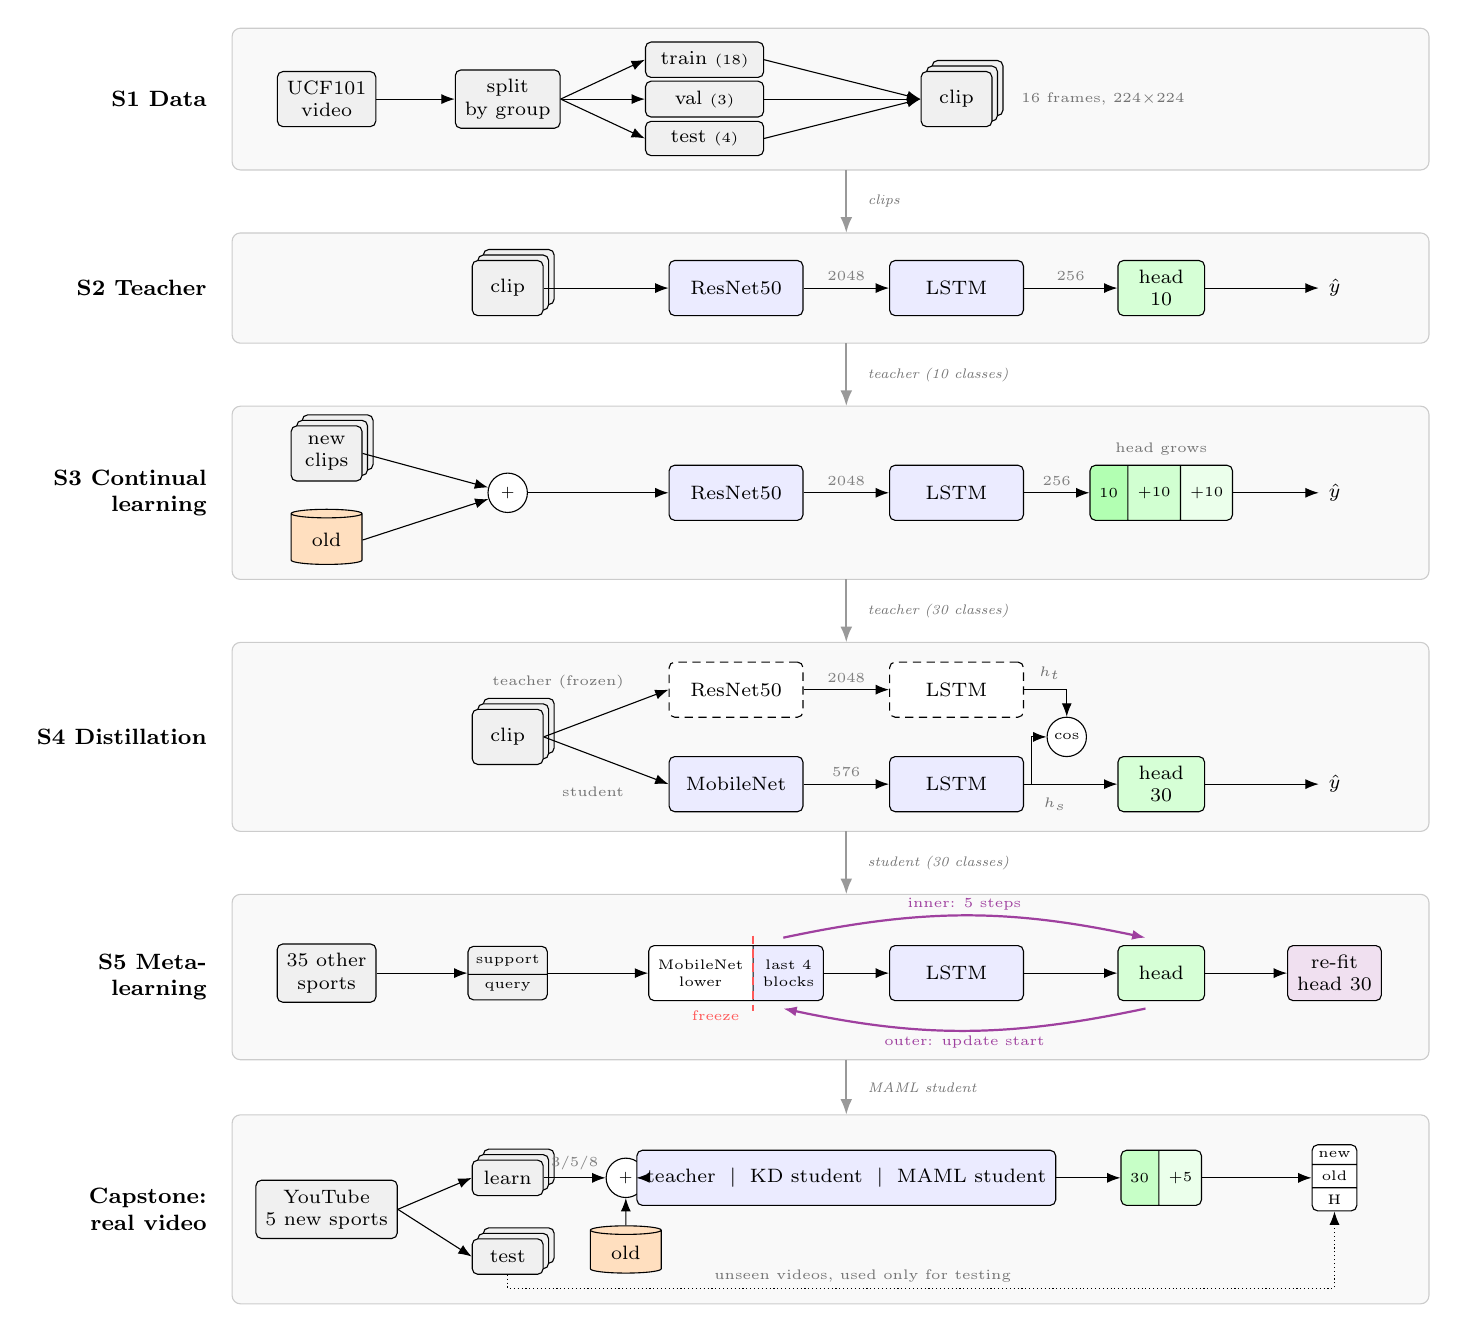
\begin{tikzpicture}[ulal]
% panels
\draw[u panel] (0, 9)    rectangle (152, -9);    \node[u stage] at (-2, 0)      {S1 Data};
\draw[u panel] (0, -17)  rectangle (152, -31);   \node[u stage] at (-2, -24)    {S2 Teacher};
\draw[u panel] (0, -39)  rectangle (152, -61);   \node[u stage] at (-2, -50)    {S3 Continual\\learning};
\draw[u panel] (0, -69)  rectangle (152, -93);   \node[u stage] at (-2, -81)    {S4 Distillation};
\draw[u panel] (0, -101) rectangle (152, -122);  \node[u stage] at (-2, -111.5) {S5 Meta-\\learning};
\draw[u panel] (0, -129) rectangle (152, -153);  \node[u stage] at (-2, -141)   {Capstone:\\real video};
\draw[u hand] (78, -9)   -- (78, -17);  \node[u handlab] at (79.5, -13)  {clips};
\draw[u hand] (78, -31)  -- (78, -39);  \node[u handlab] at (79.5, -35)  {teacher (10 classes)};
\draw[u hand] (78, -61)  -- (78, -69);  \node[u handlab] at (79.5, -65)  {teacher (30 classes)};
\draw[u hand] (78, -93)  -- (78, -101); \node[u handlab] at (79.5, -97)  {student (30 classes)};
\draw[u hand] (78, -122) -- (78, -129); \node[u handlab] at (79.5, -125.5) {MAML student};
% S1
\node[u data] (ucf) at (12, 0) {UCF101\\video};
\node[u data] (grp) at (35, 0) {split\\by group};
\node[u data, minimum height=4.3mm, minimum width=15mm] (tr) at (60, 5)  {train {\tiny(18)}};
\node[u data, minimum height=4.3mm, minimum width=15mm] (va) at (60, 0)  {val {\tiny(3)}};
\node[u data, minimum height=4.3mm, minimum width=15mm] (te) at (60, -5) {test {\tiny(4)}};
\node[u clip] (c1) at (92, 0) {clip};
\node[u small, anchor=west] at (99, 0) {16 frames, $224{\times}224$};
\draw[u arr] (ucf)--(grp);
\draw[u arr] (grp.east)--(tr.west); \draw[u arr] (grp.east)--(va.west); \draw[u arr] (grp.east)--(te.west);
\draw[u arr] (tr.east)--(c1.west); \draw[u arr] (va.east)--(c1.west); \draw[u arr] (te.east)--(c1.west);
% S2
\node[u clip] (c2) at (35, -24) {clip};
\node[u net]  (r2) at (64, -24) {ResNet50};
\node[u net]  (l2) at (92, -24) {LSTM};
\node[u head] (h2) at (118, -24) {head\\10};
\node         (y2) at (140, -24) {$\hat y$};
\draw[u arr] (c2)--(r2); \draw[u arr] (r2)--node[u dim]{2048}(l2); \draw[u arr] (l2)--node[u dim]{256}(h2); \draw[u arr] (h2)--(y2);
% S3
\node[u clip] (c3) at (12, -45) {new\\clips};
\node[u buf]  (b3) at (12, -56) {old};
\node[u op]   (p3) at (35, -50) {$+$};
\node[u net]  (r3) at (64, -50) {ResNet50};
\node[u net]  (l3) at (92, -50) {LSTM};
\node[draw, rectangle split, rectangle split horizontal, rectangle split parts=3,
      rectangle split part fill={green!30,green!18,green!8}, rounded corners=2pt,
      minimum height=7mm, font=\tiny] (h3) at (118, -50) {10\nodepart{two}+10\nodepart{three}+10};
\node[u small] at (118, -44.5) {head grows};
\node         (y3) at (140, -50) {$\hat y$};
\draw[u arr] (c3.east) -- (p3); \draw[u arr] (b3.east) -- (p3);
\draw[u arr] (p3)--(r3); \draw[u arr] (r3)--node[u dim]{2048}(l3); \draw[u arr] (l3)--node[u dim]{256}(h3); \draw[u arr] (h3)--(y3);
% S4
\node[u clip] (c4)  at (35, -81) {clip};
\node[u frz]  (r4t) at (64, -75) {ResNet50};
\node[u frz]  (l4t) at (92, -75) {LSTM};
\node[u net]  (r4s) at (64, -87) {MobileNet};
\node[u net]  (l4s) at (92, -87) {LSTM};
\node[u op]   (cos) at (106, -81) {$\cos$};
\node[u head] (h4)  at (118, -87) {head\\30};
\node         (y4)  at (140, -87) {$\hat y$};
\node[u small, anchor=east] at (51, -74) {teacher (frozen)};
\node[u small, anchor=east] at (51, -88) {student};
\draw[u arr] (c4.east)--(r4t.west); \draw[u arr] (c4.east)--(r4s.west);
\draw[u arr] (r4t)--node[u dim]{2048}(l4t); \draw[u arr] (r4s)--node[u dim]{576}(l4s);
\draw[u arr] (l4t.east) -| node[u small, pos=0.3, above]{$h_t$} (cos.north);
\draw[u arr] (l4s)--(h4); \draw[u arr] (h4)--(y4);
\draw[u arr] (101.5, -87) |- (cos.west); \node[u small] at (104.5, -89.5) {$h_s$};
% S5
\node[u data] (sp5) at (12, -111) {35 other\\sports};
\node[draw, rectangle split, rectangle split parts=2, rounded corners=2pt, fill=gray!12,
      align=center, font=\tiny, inner sep=1mm] (ep5) at (35, -111) {support\nodepart{two}query};
\node[draw, rectangle split, rectangle split horizontal, rectangle split parts=2,
      rectangle split part fill={white,blue!8}, rounded corners=2pt, minimum height=7mm,
      align=center, font=\tiny] (m5) at (64, -111) {MobileNet\\lower\nodepart{two}last 4\\blocks};
\node[u net]  (l5) at (92, -111) {LSTM};
\node[u head] (h5) at (118, -111) {head};
\node[u meta] (rf5) at (140, -111) {re-fit\\head 30};
\draw[u arr] (sp5)--(ep5); \draw[u arr] (ep5)--(m5); \draw[u arr] (m5)--(l5); \draw[u arr] (l5)--(h5); \draw[u arr] (h5)--(rf5);
\draw[red!65, densely dashed, thick] ($(m5.one split north)+(0,1.2)$) -- ($(m5.one split south)+(0,-1.2)$);
\node[font=\tiny, text=red!65, anchor=east] at ($(m5.one split south)+(-0.5,-1.8)$) {freeze};
\draw[u arr, violet!75, thick] (70, -106.5) to[bend left=12] node[font=\tiny, above=-0.6mm]{inner: 5 steps} (116, -106.5);
\draw[u arr, violet!75, thick] (116, -115.5) to[bend left=12] node[font=\tiny, below=-0.6mm]{outer: update start} (70, -115.5);
% Capstone
\node[u data] (yt) at (12, -141) {YouTube\\5 new sports};
\node[u clip, minimum height=4.5mm] (lr) at (35, -137) {learn};
\node[u clip, minimum height=4.5mm] (ts) at (35, -147) {test};
\node[u op]   (p6) at (50, -137) {$+$};
\node[u buf, minimum height=6mm] (b6) at (50, -146.5) {old};
\node[u box, fill=blue!8, minimum width=45mm] (mod6) at (78, -137) {teacher $\;|\;$ KD student $\;|\;$ MAML student};
\node[draw, rectangle split, rectangle split horizontal, rectangle split parts=2,
      rectangle split part fill={green!22,green!8}, rounded corners=2pt, minimum height=7mm,
      font=\tiny] (h6) at (118, -137) {30\nodepart{two}+5};
\node[draw, rectangle split, rectangle split parts=3, rounded corners=2pt, fill=white,
      font=\tiny, inner sep=0.8mm] (res6) at (140, -137) {new\nodepart{two}old\nodepart{three}H};
\draw[u arr] (yt.east)--(lr.west); \draw[u arr] (yt.east)--(ts.west);
\draw[u arr] (lr)--node[u dim]{3/5/8}(p6); \draw[u arr] (b6)--(p6);
\draw[u arr] (p6)--(mod6); \draw[u arr] (mod6)--(h6); \draw[u arr] (h6.east) -- (h6.east -| res6.west);
\draw[u arr, densely dotted] (ts.south) |- (140, -151) -- (res6.south);
\node[u small, anchor=west] at (60, -149.5) {unseen videos, used only for testing};
\end{tikzpicture}}
\caption{\textbf{The ULAL architecture.} One panel per stage; the grey arrows show what each
stage hands to the next. Every panel uses the winner of its study
(Sections~\ref{sec:data}--\ref{sec:meta}) and Section~\ref{sec:ulal} walks through the
whole pipeline. Grey: data; blue: trained; dashed: frozen; orange: stored old clips; violet:
meta-learning; green: classifier head; red dashed: freeze boundary.}
\label{fig:pipeline}
\end{figure*}

%------------------------------------------------------------------------------
\section{Related Work}
\textbf{Continual learning.} Approaches fall into three families.
\emph{Regularisation} methods add a penalty that discourages changing parameters
important to old tasks: EWC~\cite{kirkpatrick2017ewc} weights the penalty by the Fisher
information, and synaptic-intelligence variants use online importance
estimates~\cite{zenke2017si}. \emph{Functional} methods keep the model's outputs stable:
Learning without Forgetting (LwF)~\cite{li2017lwf} distils the old model's own
predictions on new data. \emph{Rehearsal} methods store and replay a small set of past
exemplars; iCaRL~\cite{rebuffi2017icarl} combines rehearsal with distillation. We evaluate
a representative of each family on video, where the cost of storing exemplars is a
first-order concern. \textbf{Knowledge distillation.} A compact student can be trained to
match a larger teacher's softened logits~\cite{hinton2015kd} or its intermediate
features~\cite{romero2015fitnets}; we compare logit distillation against two feature
objectives. \textbf{Meta and few-shot learning.} MAML~\cite{finn2017maml} learns an
initialisation from which a few gradient steps adapt to a new task; first-order MAML drops
the second-order term for efficiency. Few-shot class-incremental learning
(FSCIL)~\cite{tao2020fscil} adds new classes from few examples while retaining a large
base set, and reports the harmonic mean of base and new accuracy so that neither side can
be ignored; we adopt that metric.

%------------------------------------------------------------------------------
\section{System, Notation, and Protocol}
\label{sec:setup}

\subsection{The shared recogniser}
Every stage uses the same recogniser (Fig.~\ref{fig:arch}). A clip is $T{=}16$ RGB frames
at $224\times224$, ImageNet-normalised. A CNN backbone $\phi$ is applied to each frame
independently, producing frame features $\phi(x_1),\dots,\phi(x_T)$. An LSTM reads that
sequence and its final hidden state $h_T\in\mathbb{R}^{256}$ is the clip feature. A linear
head $W$ maps $h_T$ to class scores:
\begin{equation}
h_T = \mathrm{LSTM}\big(\phi(x_1),\dots,\phi(x_T)\big),\qquad z = W\,h_T .
\end{equation}
The head \emph{grows} as classes arrive: adding $k$ classes appends $k$ rows to $W$ and
keeps the existing rows. The teacher uses ResNet50 as $\phi$ (2048-d per frame), the
student MobileNetV3-Small (576-d); both use the same 256-d LSTM, so their clip features
$h$ can be compared directly.

\begin{figure}[t]
\centering
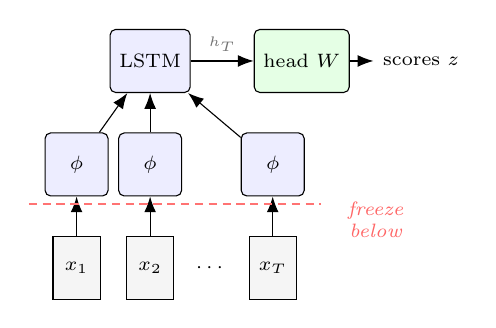
\begin{tikzpicture}[
  font=\scriptsize, node distance=3.2mm,
  fr/.style={draw, minimum width=6mm, minimum height=8mm, fill=gray!8},
  cnn/.style={draw, rounded corners=2pt, minimum width=8mm, minimum height=8mm, fill=blue!7},
  lstm/.style={draw, rounded corners=2pt, minimum width=10mm, minimum height=8mm, fill=blue!7},
  head/.style={draw, rounded corners=2pt, minimum width=9mm, minimum height=8mm, fill=green!10},
  arr/.style={-{Latex[length=2mm]}}
]
\node[fr] (f1) {$x_1$};
\node[fr, right=of f1] (f2) {$x_2$};
\node[right=1.5mm of f2] (dots) {$\cdots$};
\node[fr, right=1.5mm of dots] (fT) {$x_T$};
\node[cnn, above=5mm of f1] (c1) {$\phi$};
\node[cnn, above=5mm of f2] (c2) {$\phi$};
\node[cnn, above=5mm of fT] (cT) {$\phi$};
\node[lstm, above=5mm of c2] (lstm) {LSTM};
\node[head, right=8mm of lstm] (head) {head $W$};
\node[right=3mm of head] (out) {scores $z$};
\draw[arr] (f1)--(c1); \draw[arr] (f2)--(c2); \draw[arr] (fT)--(cT);
\draw[arr] (c1)--(lstm); \draw[arr] (c2)--(lstm); \draw[arr] (cT)--(lstm);
\draw[arr] (lstm)--node[above, font=\tiny, text=black!55]{$h_T$}(head); \draw[arr] (head)--(out);
\draw[densely dashed, red!55, thick] ($(c1.south west)+(-2mm,-1mm)$) -- ($(cT.south east)+(2mm,-1mm)$);
\node[font=\scriptsize\itshape, text=red!60, align=center] at ($(cT.south east)+(9mm,-3mm)$)
  {freeze\\below};
\end{tikzpicture}
\caption{\textbf{The shared recogniser.} The backbone $\phi$ runs on each of the 16 frames;
an LSTM summarises them into a 256-d clip feature $h_T$; a growing head classifies. The
freeze boundary (dashed) marks how deep training may reach in a stage.}
\label{fig:arch}
\end{figure}

\subsection{The moving freeze boundary}
The stages differ in \emph{which} parameters they train. Stage~2 trains the whole
recogniser. Stage~3 trains the whole recogniser again for each new task (every method in
that study trains the same parameters), and the head grows. Stage~4 freezes the teacher
and trains the whole student. Stage~5 freezes the lower student backbone and meta-trains
only its last four blocks, the LSTM, and the head, so the old features are protected while
the upper layers reshape. Within a stage every compared method trains the \emph{same}
parameters, so only the mechanism under test differs.

\subsection{Datasets and budget}
All experiments use UCF101 on one free Colab T4 GPU. The group-disjoint split assigns
whole source groups to one split, 18/3/4 groups per class (train/val/test), keeping the
usual $\approx$72/12/16\% proportions (Section~\ref{sec:data}). Table~\ref{tab:hparams}
lists the budget of each stage; seeds are fixed and reset before every training run.

\begin{table}[t]
\centering
\caption{Budget per stage (shared by every method compared in that stage).}
\label{tab:hparams}
\renewcommand{\arraystretch}{1.12}
\begin{tabular}{ll}
\toprule
Stage & Key settings \\
\midrule
Backbone (S2)     & Adam, lr $10^{-4}$, 5 epochs \\
Continual (S3)    & Adam, lr $10^{-4}$, 5 epochs/task; replay 15/class; \\
                  & LwF weight 3.0, $T{=}5$; EWC $\lambda{=}2800$ \\
Distillation (S4) & Adam, lr $10^{-4}$, 15 epochs; \\
                  & $T{=}2$; CE/transfer $0.75/0.25$ \\
Meta-train (S5)   & 5-way 3-shot, 60 episodes $\times$ 8 epochs; \\
                  & 40 sports; inner SGD 5 steps @ $0.05$; \\
                  & meta-lr $10^{-4}$; last 4 blocks trained \\
Adaptation (S5)   & 8 clips/class, 5 epochs, lr $3\!\times\!10^{-4}$; \\
                  & replay 8/class; LwF $0.5$, $T{=}2$ \\
Capstone          & replay 15/class ($10\!\to\!20\!\to\!30$); \\
                  & cosine KD, 10 epochs; \\
                  & MAML 5-way 3-shot, 35 sports (1 clip/video); \\
                  & YouTube: 3/5/8 clips, 5 epochs, \\
                  & lr $3\!\times\!10^{-4}$, replay 8/class \\
\bottomrule
\end{tabular}
\end{table}

\subsection{How to read the numbers}
\emph{Test accuracy} is the fraction correct on the unseen, group-disjoint test set.
\emph{Old} and \emph{New} split it into classes learned earlier and the newest task;
\emph{Base} is retention on the original classes. When old classes outnumber new ones, a
plain average mostly measures the old side and rewards a method that learns nothing new, so
for few-shot learning we also report the harmonic mean
\begin{equation}
\label{eq:harm}
\mathrm{H}=\frac{2\,\mathrm{acc}_{\text{new}}\,\mathrm{acc}_{\text{old}}}
{\mathrm{acc}_{\text{new}}+\mathrm{acc}_{\text{old}}},
\end{equation}
which is high only when \emph{both} sides are high~\cite{tao2020fscil}.

%------------------------------------------------------------------------------
\section{Stage 1 --- Data Split and Leakage}
\label{sec:data}
\textbf{Why this comes first.} A UCF101 filename \texttt{v\_Class\_gXX\_cYY.avi} encodes a
\emph{group} \texttt{gXX} (one source recording) and a \emph{clip} \texttt{cYY} (one segment
of it). All clips of a group share the same actor, background and camera. If the split is
made per clip, segments of the \emph{same} recording land in train and test, and the model
can recognise the \emph{scene} instead of the \emph{action}. We therefore assign each whole
group to a single split (panel S1 of Fig.~\ref{fig:pipeline}).

\begin{table}[t]
\centering
\caption{Source groups shared between splits (20 studied classes, 2{,}679 videos).}
\label{tab:leak}
\renewcommand{\arraystretch}{1.1}
\begin{tabular}{lccc}
\toprule
Split & Groups & Groups in $>$1 split & Leak \\
\midrule
Shipped (per clip)        & 500 & 400 & 80\% \\
\textbf{Group-disjoint}   & 500 & 0   & \textbf{0\%} \\
\bottomrule
\end{tabular}
\end{table}

\textbf{Result and reading.} Table~\ref{tab:leak}: the shipped split puts 400 of 500
groups in more than one split, so 80\% of the test recordings were partly seen in
training; the group-disjoint split puts none. It keeps the usual 72/12/16\% proportions,
so every later accuracy is lower than commonly reported on UCF101 only because the
inflation is gone---and since the same leak would inflate every later stage, fixing it
once at the source makes the whole study trustworthy.

%------------------------------------------------------------------------------
\section{Stage 2 --- Backbone Selection}
\label{sec:backbone}
\textbf{Design.} The backbone $\phi$ is the only part that changes: each candidate is
plugged into the same recogniser (clip $\to\phi\to$ LSTM $\to$ head, panel S2 of
Fig.~\ref{fig:pipeline}) and trained with the same budget and seed. We expect a network
with no prior knowledge (a CNN trained from scratch) to struggle on a few thousand clips,
and ImageNet-pretrained networks to cluster high.

\begin{table}[t]
\centering
\caption{Backbone bake-off on the 10 base classes (group-disjoint test).}
\label{tab:backbone}
\renewcommand{\arraystretch}{1.1}
\begin{tabular}{lccc}
\toprule
Backbone $\phi$ & Test acc.\ (\%) & Params (M) & ms/clip \\
\midrule
ScratchCNN        & 52.8 & 103.1 & 10.2 \\
ResNet18          & 90.1 & 12.0 & 15.7 \\
DenseNet121       & 92.0 & 8.3  & 53.1 \\
VGG19-BN          & 92.0 & 20.8 & 115.7 \\
\textbf{ResNet50 (selected)} & \textbf{93.9} & 25.9 & 54.6 \\
\bottomrule
\end{tabular}
\end{table}

\textbf{Result and why.} Table~\ref{tab:backbone}. The from-scratch CNN has the most
parameters (103M, because its LSTM reads a large flattened feature map) yet the worst
accuracy (52.8\%): capacity without useful priors does not help on little data. All four
pretrained backbones exceed 90\%, because the hard part---good spatial features---is solved
before the LSTM sees anything. \textbf{ResNet50 is selected}: it is the most accurate
(93.9\%), its 2048-d feature gives the later stages the richest representation, and at
55~ms per clip it is half as slow as VGG19-BN.

%------------------------------------------------------------------------------
\section{Stage 3 --- Continual Learning}
\label{sec:cl}
\textbf{Design.} Starting from the 10-class teacher, the head grows and the model learns
two new tasks, $10\!\to\!15\!\to\!20$ classes. The five methods of Fig.~\ref{fig:cl} train
the same network with the same budget; they differ only in \emph{what protects the old
classes}. Writing $\mathcal{L}_{\text{CE}}$ for cross-entropy on the batch:
\begin{itemize}
\item \textbf{S3.0 Naive}: $\mathcal{L}=\mathcal{L}_{\text{CE}}(\text{new})$ --- nothing
protects the past.
\item \textbf{S3.1 EWC}~\cite{kirkpatrick2017ewc}: adds
$\tfrac{\lambda}{2}\sum_i F_i(\theta_i-\theta_i^{\star})^2$, a penalty that keeps the
weights $\theta$ important for old classes (Fisher $F_i$) near their old values
$\theta^\star$.
\item \textbf{S3.2 LwF}~\cite{li2017lwf}: adds
$\lambda\,\mathrm{KD}\big(z_{1:C_{\text{old}}},\,z^{\star}_{1:C_{\text{old}}}\big)$, keeping
the old-class scores of the new model close to those of a frozen copy of the old model,
computed on the new clips.
\item \textbf{S3.3 Replay}: stores 15 old clips per class and mixes them 1:1 into every
new batch, $\mathcal{L}=\mathcal{L}_{\text{CE}}(\text{new}\cup\text{old})$.
\item \textbf{S3.4 Replay+LwF}~\cite{rebuffi2017icarl}: both.
\end{itemize}

% ============================ FIG. 3: CL METHODS ============================
\begin{figure*}[t]
\centering
\resizebox{\textwidth}{!}{%
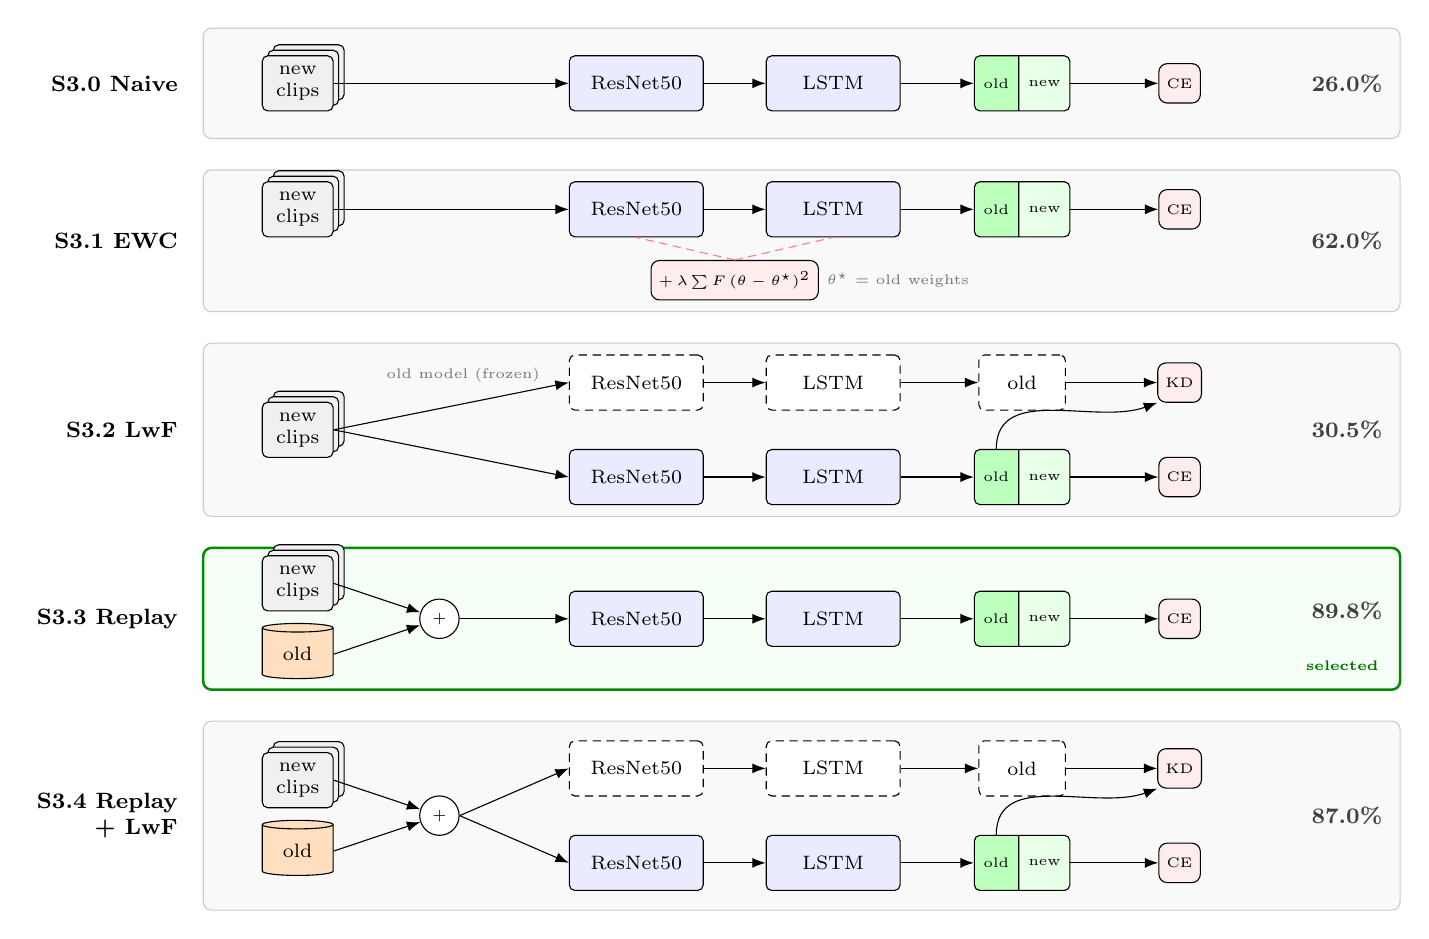
\begin{tikzpicture}[ulal]
% ---- S3.0 Naive ----
\draw[u panel] (0, 0) rectangle (152, -14);   \node[u stage] at (-2, -7) {S3.0 Naive};
\node[u clip] (a0) at (12, -7) {new\\clips};
\node[u net]  (a1) at (55, -7) {ResNet50};
\node[u net]  (a2) at (80, -7) {LSTM};
\headsplit{a3}{104,-7}{old}{new}
\node[u loss] (a4) at (124, -7) {CE};
\node[u res] at (151, -7) {26.0\%};
\draw[u arr] (a0)--(a1); \draw[u arr] (a1)--(a2); \draw[u arr] (a2)--(a3); \draw[u arr] (a3)--(a4);
% ---- S3.1 EWC ----
\draw[u panel] (0, -18) rectangle (152, -36); \node[u stage] at (-2, -27) {S3.1 EWC};
\node[u clip] (b0) at (12, -23) {new\\clips};
\node[u net]  (b1) at (55, -23) {ResNet50};
\node[u net]  (b2) at (80, -23) {LSTM};
\headsplit{b3}{104,-23}{old}{new}
\node[u loss] (b4) at (124, -23) {CE};
\node[u loss] (b5) at (67.5, -32) {$+\,\lambda\sum F\,(\theta-\theta^{\star})^2$};
\node[u small, anchor=west] at (78, -32) {$\theta^{\star}$ = old weights};
\node[u res] at (151, -27) {62.0\%};
\draw[u arr] (b0)--(b1); \draw[u arr] (b1)--(b2); \draw[u arr] (b2)--(b3); \draw[u arr] (b3)--(b4);
\draw[densely dashed, red!50] (b5.north) -- (b1.south); \draw[densely dashed, red!50] (b5.north) -- (b2.south);
% ---- S3.2 LwF ----
\draw[u panel] (0, -40) rectangle (152, -62); \node[u stage] at (-2, -51) {S3.2 LwF};
\node[u clip] (c0) at (12, -51) {new\\clips};
\node[u frz]  (c1t) at (55, -45) {ResNet50};
\node[u frz]  (c2t) at (80, -45) {LSTM};
\node[u box, densely dashed, fill=white, minimum width=11mm] (c3t) at (104, -45) {old};
\node[u net]  (c1) at (55, -57) {ResNet50};
\node[u net]  (c2) at (80, -57) {LSTM};
\headsplit{c3}{104,-57}{old}{new}
\node[u loss] (c4) at (124, -57) {CE};
\node[u loss] (c5) at (124, -45) {KD};
\node[u small, anchor=east] at (44, -44) {old model (frozen)};
\node[u res] at (151, -51) {30.5\%};
\draw[u arr] (c0.east)--(c1t.west); \draw[u arr] (c0.east)--(c1.west);
\draw[u arr] (c1t)--(c2t); \draw[u arr] (c2t)--(c3t); \draw[u arr] (c3t)--(c5);
\draw[u arr] (c1)--(c2); \draw[u arr] (c2)--(c3); \draw[u arr] (c3)--(c4);
\draw[u arr] (c3.one north) to[out=90, in=200] (c5.south west);
% ---- S3.3 Replay (selected) ----
\draw[u best] (0, -66) rectangle (152, -84);  \node[u stage] at (-2, -75) {S3.3 Replay};
\node[u pick] at (150.5, -81) {selected};
\node[u clip] (d0) at (12, -70.5) {new\\clips};
\node[u buf]  (d5) at (12, -79.5) {old};
\node[u op]   (d6) at (30, -75) {$+$};
\node[u net]  (d1) at (55, -75) {ResNet50};
\node[u net]  (d2) at (80, -75) {LSTM};
\headsplit{d3}{104,-75}{old}{new}
\node[u loss] (d4) at (124, -75) {CE};
\node[u res] at (151, -74) {89.8\%};
\draw[u arr] (d0.east)--(d6); \draw[u arr] (d5.east)--(d6);
\draw[u arr] (d6)--(d1); \draw[u arr] (d1)--(d2); \draw[u arr] (d2)--(d3); \draw[u arr] (d3)--(d4);
% ---- S3.4 Replay + LwF ----
\draw[u panel] (0, -88) rectangle (152, -112); \node[u stage] at (-2, -100) {S3.4 Replay\\+ LwF};
\node[u clip] (e0) at (12, -95.5) {new\\clips};
\node[u buf]  (e5) at (12, -104.5) {old};
\node[u op]   (e6) at (30, -100) {$+$};
\node[u frz]  (e1t) at (55, -94) {ResNet50};
\node[u frz]  (e2t) at (80, -94) {LSTM};
\node[u box, densely dashed, fill=white, minimum width=11mm] (e3t) at (104, -94) {old};
\node[u net]  (e1) at (55, -106) {ResNet50};
\node[u net]  (e2) at (80, -106) {LSTM};
\headsplit{e3}{104,-106}{old}{new}
\node[u loss] (e4) at (124, -106) {CE};
\node[u loss] (e7) at (124, -94) {KD};
\node[u res] at (151, -100) {87.0\%};
\draw[u arr] (e0.east)--(e6); \draw[u arr] (e5.east)--(e6);
\draw[u arr] (e6.east)--(e1t.west); \draw[u arr] (e6.east)--(e1.west);
\draw[u arr] (e1t)--(e2t); \draw[u arr] (e2t)--(e3t); \draw[u arr] (e3t)--(e7);
\draw[u arr] (e1)--(e2); \draw[u arr] (e2)--(e3); \draw[u arr] (e3)--(e4);
\draw[u arr] (e3.one north) to[out=90, in=200] (e7.south west);
\end{tikzpicture}}
\caption{\textbf{Stage 3: the five continual-learning methods.} All train the same
network (blue) with a head that grows by the new classes; they differ only in what
protects the old classes: nothing (S3.0), a weight penalty (S3.1), the scores of a frozen
copy of the old model (S3.2, dashed), stored old clips (S3.3, orange), or both (S3.4). Right:
final accuracy on all 20 classes (Table~\ref{tab:cl}). Replay is used in the pipeline.}
\label{fig:cl}
\end{figure*}

\begin{table}[t]
\centering
\caption{Continual learning after the full $10\!\to\!15\!\to\!20$ stream (\%). Final: all
20 classes; Old: classes 0--14; New: last task 15--19; Base: original 10.}
\label{tab:cl}
\renewcommand{\arraystretch}{1.1}
\begin{tabular}{lcccc}
\toprule
Method & Final & Old (0--14) & New (15--19) & Base (0--9) \\
\midrule
S3.0 Naive             & 26.0 & 0.9  & 94.9 & 0.5 \\
S3.2 LwF               & 30.5 & 5.3  & 100.0 & 0.0 \\
S3.1 EWC               & 62.0 & 71.1 & 36.8 & 76.9 \\
S3.4 Replay+LwF        & 87.0 & 82.6 & 99.2 & 83.0 \\
\textbf{S3.3 Replay}   & \textbf{89.8} & 86.7 & 98.3 & 89.2 \\
\bottomrule
\end{tabular}
\end{table}

\begin{table}[t]
\centering
\caption{When each method forgets: accuracy per task (\%) after learning task~1 and after
learning task~2. Before any new task the base accuracy is 93.9.}
\label{tab:cltime}
\renewcommand{\arraystretch}{1.1}
\setlength{\tabcolsep}{4.5pt}
\begin{tabular}{lccccc}
\toprule
 & \multicolumn{2}{c}{after task 1} & \multicolumn{3}{c}{after task 2} \\
\cmidrule(lr){2-3}\cmidrule(lr){4-6}
Method & Base & Task 1 & Base & Task 1 & Task 2 \\
\midrule
S3.0 Naive       & 22.6 & 98.2 & 0.5  & 1.8  & 94.9 \\
S3.1 EWC         & 80.7 & 79.1 & 76.9 & 60.0 & 36.8 \\
S3.2 LwF         & 26.4 & 97.3 & 0.0  & 15.5 & 100.0 \\
S3.3 Replay      & 89.6 & 94.6 & 89.2 & 81.8 & 98.3 \\
S3.4 Replay+LwF  & 87.3 & 96.4 & 83.0 & 81.8 & 99.2 \\
\bottomrule
\end{tabular}
\end{table}

\textbf{Results.} Table~\ref{tab:cl} gives the final accuracies and
Table~\ref{tab:cltime} shows \emph{when} each method forgets.

\textbf{Why each method behaves as it does.}
\emph{S3.0 Naive} learns every new task almost perfectly (98.2\% on task~1, 94.9\% on
task~2) but the base falls from 93.9\% to 22.6\% after one task and to 0.5\% after two:
with only new labels in every batch, the shared weights are rewritten for the newest task.
\emph{S3.2 LwF} forgets almost as much (base 26.4\% $\to$ 0.0\%) even though it protects the
old scores. The reason is the setting: the original LwF~\cite{li2017lwf} gives every task
its own head and is tested with the task known, whereas here one head covers all classes
and the task is not known at test time. The distillation term only keeps the \emph{ranking
among old classes}, while the cross-entropy on new clips keeps raising the new classes
above all old ones; the old clips are then out-voted by the newest classes---in the
confusion matrices almost every forgotten base clip is predicted as a \emph{new} class,
not as another old one. \emph{S3.1 EWC} fails the other way: its penalty keeps the base
(76.9\%) but also blocks the new task (36.8\% on task~2), a stability/plasticity lock.
\emph{S3.3 Replay} is the only method that keeps every task high (base 89.2\%, task~1
81.8\%, task~2 98.3\%): the stored clips come with their old labels, so every batch also
tells the model what the old classes look like and puts them back in the competition.
\emph{S3.4 Replay+LwF} is close (87.0\%) but slightly lower: the buffer already protects
the old classes, and the extra distillation term only slows the new task.
\textbf{Choice for the pipeline: replay} (panel S3 of Fig.~\ref{fig:pipeline}). On video,
storing a few clips beats every data-free method.

%------------------------------------------------------------------------------
\section{Stage 4 --- Knowledge Distillation}
\label{sec:kd}
\textbf{Design.} The 25.9M-parameter teacher is too big for a small device, so we train a
MobileNetV3-Small+LSTM student ($\approx$1.8M parameters, $14\times$ smaller). The four
objectives of Fig.~\ref{fig:kd} share the student, data, budget and seed, and all use
$\mathcal{L}=0.75\,\mathcal{L}_{\text{CE}}+0.25\,\mathcal{L}_{\text{transfer}}$:
\begin{itemize}
\item \textbf{S4.0 CE only}: $\mathcal{L}_{\text{transfer}}=0$ (no teacher, the baseline).
\item \textbf{S4.1 KD}~\cite{hinton2015kd}: match the teacher's softened scores,
$T^2\,\mathrm{KL}\big(\sigma(z_t/T)\,\|\,\sigma(z_s/T)\big)$, $T=2$.
\item \textbf{S4.2 Cosine}: align the 256-d clip features by direction,
$1-\cos(h_s,h_t)$.
\item \textbf{S4.3 MSE}~\cite{romero2015fitnets}: a learnable regressor $g$ maps $h_s$ onto
the teacher's feature before an $\ell_2$ match, $\lVert g(h_s)-h_t\rVert_2^2$ ($g$ is
dropped at inference).
\end{itemize}

% ============================ FIG. 4: KD OBJECTIVES ============================
\begin{figure*}[t]
\centering
\resizebox{\textwidth}{!}{%
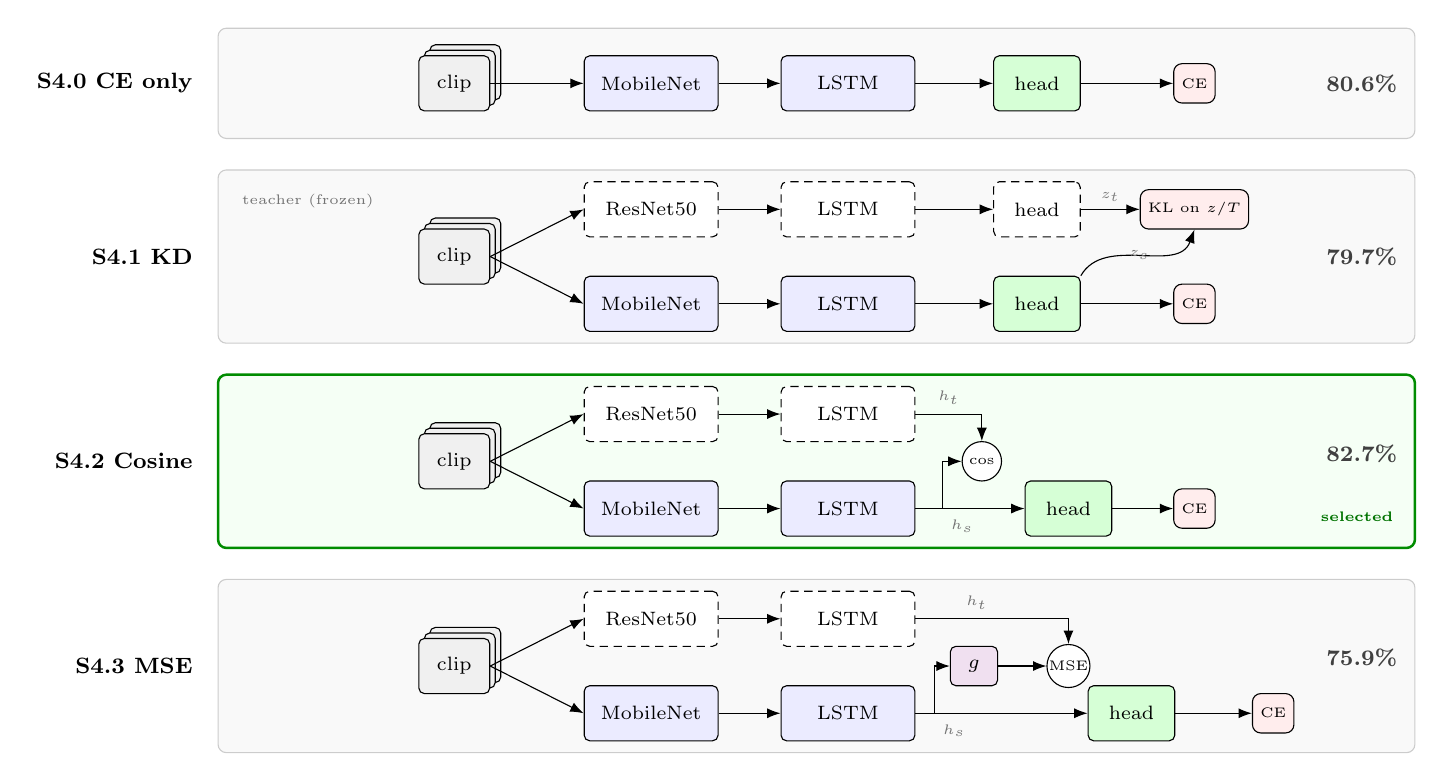
\begin{tikzpicture}[ulal]
% ---- S4.0 CE only ----
\draw[u panel] (0, 0) rectangle (152, -14);  \node[u stage] at (-2, -7) {S4.0 CE only};
\node[u clip] (a0) at (30, -7) {clip};
\node[u net]  (a1) at (55, -7) {MobileNet};
\node[u net]  (a2) at (80, -7) {LSTM};
\node[u head] (a3) at (104, -7) {head};
\node[u loss] (a4) at (124, -7) {CE};
\node[u res] at (151, -7) {80.6\%};
\draw[u arr] (a0)--(a1); \draw[u arr] (a1)--(a2); \draw[u arr] (a2)--(a3); \draw[u arr] (a3)--(a4);
% ---- S4.1 KD (logits) ----
\draw[u panel] (0, -18) rectangle (152, -40); \node[u stage] at (-2, -29) {S4.1 KD};
\node[u clip] (b0) at (30, -29) {clip};
\node[u frz]  (b1t) at (55, -23) {ResNet50};
\node[u frz]  (b2t) at (80, -23) {LSTM};
\node[u box, densely dashed, fill=white, minimum width=11mm] (b3t) at (104, -23) {head};
\node[u net]  (b1) at (55, -35) {MobileNet};
\node[u net]  (b2) at (80, -35) {LSTM};
\node[u head] (b3) at (104, -35) {head};
\node[u loss] (b4) at (124, -35) {CE};
\node[u loss] (b5) at (124, -23) {KL on $z/T$};
\node[u small, anchor=east] at (21, -22) {teacher (frozen)};
\node[u res] at (151, -29) {79.7\%};
\draw[u arr] (b0.east)--(b1t.west); \draw[u arr] (b0.east)--(b1.west);
\draw[u arr] (b1t)--(b2t); \draw[u arr] (b2t)--(b3t); \draw[u arr] (b3t)--node[u dim]{$z_t$}(b5);
\draw[u arr] (b1)--(b2); \draw[u arr] (b2)--(b3); \draw[u arr] (b3)--(b4);
\draw[u arr] (b3.north east) to[out=60, in=250] node[u small, pos=0.35, right]{$z_s$} (b5.south);
% ---- S4.2 Cosine (selected) ----
\draw[u best] (0, -44) rectangle (152, -66);  \node[u stage] at (-2, -55) {S4.2 Cosine};
\node[u pick] at (150.5, -62) {selected};
\node[u clip] (c0) at (30, -55) {clip};
\node[u frz]  (c1t) at (55, -49) {ResNet50};
\node[u frz]  (c2t) at (80, -49) {LSTM};
\node[u net]  (c1) at (55, -61) {MobileNet};
\node[u net]  (c2) at (80, -61) {LSTM};
\node[u head] (c3) at (108, -61) {head};
\node[u loss] (c4) at (124, -61) {CE};
\node[u op]   (c5) at (97, -55) {$\cos$};
\node[u res] at (151, -54) {82.7\%};
\draw[u arr] (c0.east)--(c1t.west); \draw[u arr] (c0.east)--(c1.west);
\draw[u arr] (c1t)--(c2t); \draw[u arr] (c2t.east) -| node[u small, pos=0.25, above]{$h_t$} (c5.north);
\draw[u arr] (c1)--(c2); \draw[u arr] (c2)--(c3); \draw[u arr] (c3)--(c4);
\draw[u arr] (92, -61) |- (c5.west); \node[u small] at (94.5, -63.2) {$h_s$};
% ---- S4.3 MSE with regressor ----
\draw[u panel] (0, -70) rectangle (152, -92); \node[u stage] at (-2, -81) {S4.3 MSE};
\node[u clip] (d0) at (30, -81) {clip};
\node[u frz]  (d1t) at (55, -75) {ResNet50};
\node[u frz]  (d2t) at (80, -75) {LSTM};
\node[u net]  (d1) at (55, -87) {MobileNet};
\node[u net]  (d2) at (80, -87) {LSTM};
\node[u head] (d3) at (116, -87) {head};
\node[u loss] (d4) at (134, -87) {CE};
\node[u meta, minimum height=5mm, minimum width=6mm, inner sep=0.6mm] (d6) at (96, -81) {$g$};
\node[u op]   (d5) at (108, -81) {MSE};
\node[u res] at (151, -80) {75.9\%};
\draw[u arr] (d0.east)--(d1t.west); \draw[u arr] (d0.east)--(d1.west);
\draw[u arr] (d1t)--(d2t); \draw[u arr] (d2t.east) -| node[u small, pos=0.2, above]{$h_t$} (d5.north);
\draw[u arr] (d1)--(d2); \draw[u arr] (d2)--(d3); \draw[u arr] (d3)--(d4);
\draw[u arr] (91, -87) |- (d6.west); \draw[u arr] (d6)--(d5);
\node[u small] at (93.5, -89.2) {$h_s$};
\end{tikzpicture}}
\caption{\textbf{Stage 4: the four distillation objectives.} The student (blue) always
learns from the labels (CE); the frozen teacher (dashed) adds nothing (S4.0), its softened
scores (S4.1), its clip feature by direction (S4.2), or its clip feature through a
learnable regressor $g$ (S4.3). Right: student test accuracy (Table~\ref{tab:kd}). Cosine
is used in the pipeline.}
\label{fig:kd}
\end{figure*}

\begin{table}[t]
\centering
\caption{Distillation into the MobileNetV3-Small student (20-class group-disjoint test).
Same student, budget, seed and initialisation; only the transfer term differs.}
\label{tab:kd}
\renewcommand{\arraystretch}{1.1}
\begin{tabular}{lcc}
\toprule
Model & Test acc.\ (\%) & Params (M) \\
\midrule
Teacher (ResNet50, Replay+LwF)  & 87.0 & 25.9 \\
S4.0 Student, CE only           & 80.6 & 1.8 \\
S4.1 Student, CE + KD           & 79.7 & 1.8 \\
\textbf{S4.2 Student, CE + cosine} & \textbf{82.7} & 1.8 \\
S4.3 Student, CE + MSE ($g$)    & 75.9 & 1.8 \\
\bottomrule
\end{tabular}
\end{table}

\textbf{Results and why.} Table~\ref{tab:kd}. The first lesson is \emph{compression}: a
student $14\times$ smaller stays within 4.3 points of its teacher (82.7\% vs 87.0\%),
because the teacher's decision function transfers. The second is the ranking of the
objectives, which follows from what each one asks of the student. \emph{S4.0 CE only} is
already strong (80.6\%): the student backbone is ImageNet-pretrained, so labels alone carry
it far. \emph{S4.1 KD} does not help here (79.7\%): the softened teacher scores add little
beyond the labels once the student is pretrained. \emph{S4.2 Cosine} is best (82.7\%, +2.1
over CE): it asks only that the student's 256-d clip feature \emph{point in the same
direction} as the teacher's, a gentle target that transfers the teacher's temporal summary
without forcing its scale. \emph{S4.3 MSE} is worst (75.9\%): it asks the student to match
direction \emph{and} magnitude across two very different backbones, a target that
fights the label loss. The gap between the objectives is modest (single seed, 439 test
clips), so the headline of this stage is compression, with cosine as the best transfer
term. \textbf{Choice for the pipeline: cosine distillation} (panel S4 of
Fig.~\ref{fig:pipeline}).

%------------------------------------------------------------------------------
\section{Stage 5 --- Few-Shot Meta-Adaptation}
\label{sec:meta}
\textbf{Design.} Given the 20-class student, how well can it learn \emph{five brand-new
sports} from only a few clips? Every arm uses the same adaptation---the same 8 clips per
new sport, 5 epochs, learning rate and seed, a head grown from 20 to 25 classes---so only
two things vary (Fig.~\ref{fig:meta}): the \emph{starting point} and the \emph{protection}
of the old classes. The three starting points are:
\begin{itemize}
\item \textbf{S5.0 Plain}: the distilled student as it is.
\item \textbf{S5.1 Fine-tune}: the student after ordinary supervised training on 40 other
sports. This is the control: it sees the same extra data as MAML.
\item \textbf{S5.2 MAML}~\cite{finn2017maml}: the student after first-order MAML on the
same 40 sports. Each episode draws 5 sports with 3 support and 3 query clips; the
\emph{inner} loop adapts a copy on the support clips,
$\theta'=\theta-\alpha\nabla_\theta\mathcal{L}^{\text{sup}}(\theta)$ (5 SGD steps), and the
\emph{outer} loop moves the start by the loss of the adapted copy on the query clips,
$\theta\leftarrow\theta-\beta\nabla_{\theta'}\mathcal{L}^{\text{qry}}(\theta')$.
\end{itemize}
For S5.1 and S5.2 only the last four backbone blocks, the LSTM and the head are trained,
and a fresh 20-class head is then re-fitted to the new features (a short linear probe on
12 clips per class). Each start is adapted with no protection, with replay (8 old clips per
class), or with replay+LwF, giving nine arms ranked by the harmonic mean of
Eq.~\eqref{eq:harm}.

% ============================ FIG. 5: META-ADAPTATION ============================
\begin{figure*}[t]
\centering
\resizebox{\textwidth}{!}{%
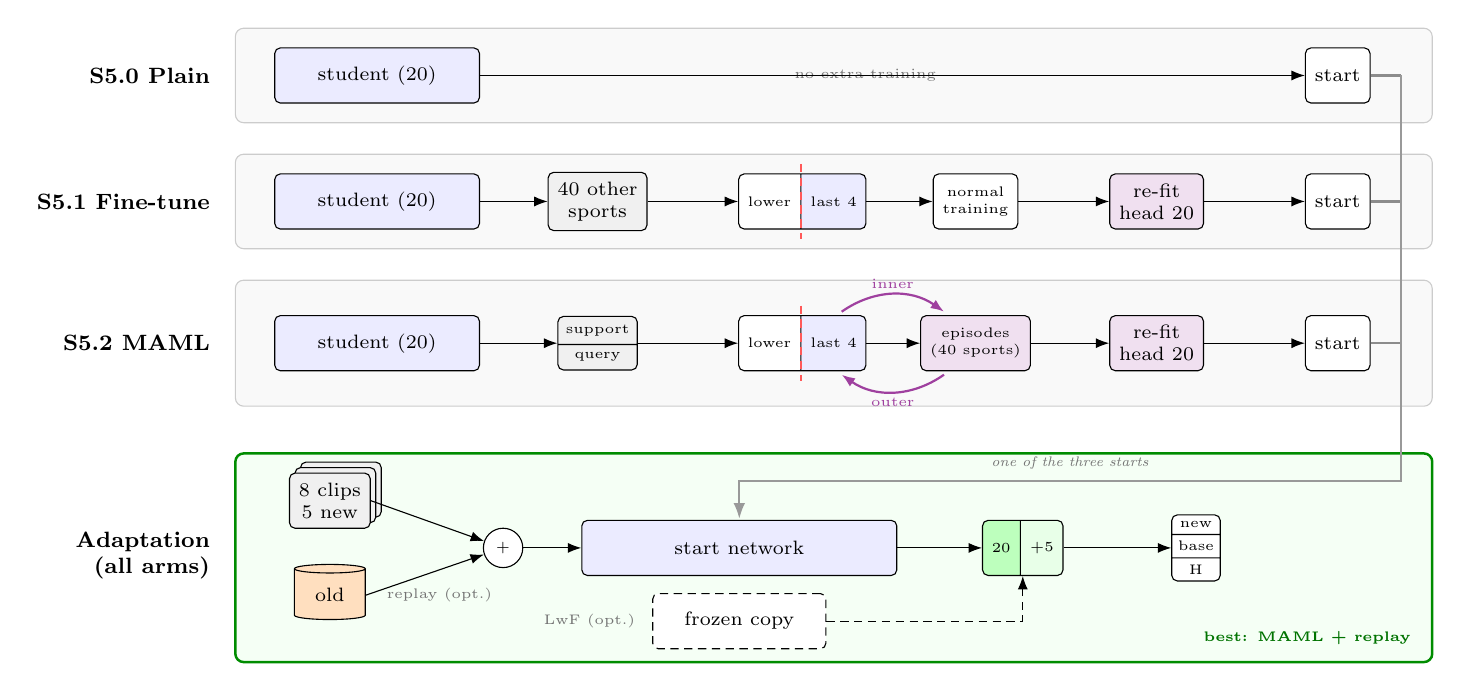
\begin{tikzpicture}[ulal]
% ---- S5.0 plain start ----
\draw[u panel] (0, 0) rectangle (152, -12);  \node[u stage] at (-2, -6) {S5.0 Plain};
\node[u net, minimum width=26mm] (a0) at (18, -6) {student (20)};
\node[u small, fill=black!2.5, inner sep=0.8pt] at (80, -6) {no extra training};
\node[u box, fill=white] (a9) at (140, -6) {start};
\draw[u arr] (a0)--(a9);
% ---- S5.1 fine-tune start ----
\draw[u panel] (0, -16) rectangle (152, -28); \node[u stage] at (-2, -22) {S5.1 Fine-tune};
\node[u net, minimum width=26mm] (b0) at (18, -22) {student (20)};
\node[u data] (b1) at (46, -22) {40 other\\sports};
\node[draw, rectangle split, rectangle split horizontal, rectangle split parts=2,
      rectangle split part fill={white,blue!8}, rounded corners=2pt, minimum height=7mm,
      align=center, font=\tiny] (b2) at (72, -22) {lower\nodepart{two}last 4};
\node[u box, fill=white, font=\tiny] (b3) at (94, -22) {normal\\training};
\node[u meta] (b4) at (117, -22) {re-fit\\head 20};
\node[u box, fill=white] (b9) at (140, -22) {start};
\draw[u arr] (b0)--(b1); \draw[u arr] (b1)--(b2); \draw[u arr] (b2)--(b3); \draw[u arr] (b3)--(b4); \draw[u arr] (b4)--(b9);
\draw[red!65, densely dashed, thick] ($(b2.one split north)+(0,1.2)$) -- ($(b2.one split south)+(0,-1.2)$);
% ---- S5.2 MAML start ----
\draw[u panel] (0, -32) rectangle (152, -48); \node[u stage] at (-2, -40) {S5.2 MAML};
\node[u net, minimum width=26mm] (c0) at (18, -40) {student (20)};
\node[draw, rectangle split, rectangle split parts=2, rounded corners=2pt, fill=gray!12,
      align=center, font=\tiny, inner sep=1mm] (c1) at (46, -40) {support\nodepart{two}query};
\node[draw, rectangle split, rectangle split horizontal, rectangle split parts=2,
      rectangle split part fill={white,blue!8}, rounded corners=2pt, minimum height=7mm,
      align=center, font=\tiny] (c2) at (72, -40) {lower\nodepart{two}last 4};
\node[u meta, font=\tiny] (c3) at (94, -40) {episodes\\(40 sports)};
\node[u meta] (c4) at (117, -40) {re-fit\\head 20};
\node[u box, fill=white] (c9) at (140, -40) {start};
\draw[u arr] (c0)--(c1); \draw[u arr] (c1)--(c2); \draw[u arr] (c2)--(c3); \draw[u arr] (c3)--(c4); \draw[u arr] (c4)--(c9);
\draw[red!65, densely dashed, thick] ($(c2.one split north)+(0,1.2)$) -- ($(c2.one split south)+(0,-1.2)$);
\draw[u arr, violet!75, thick] (77, -36) to[bend left=35] node[font=\tiny, above=-0.5mm]{inner} (90, -36);
\draw[u arr, violet!75, thick] (90, -44) to[bend left=35] node[font=\tiny, below=-0.5mm]{outer} (77, -44);
% ---- shared adaptation ----
\draw[u best] (0, -54) rectangle (152, -80.5); \node[u stage] at (-2, -67) {Adaptation\\(all arms)};
\draw[black!45, thick] (a9.east) -- (148, -6); \draw[black!45, thick] (b9.east) -- (148, -22); \draw[black!45, thick] (c9.east) -- (148, -40);
\draw[u hand] (148, -6) -- (148, -57.5) -- (64, -57.5) -- (64, -62.3);
\node[u handlab, anchor=south] at (106, -57.3) {one of the three starts};
\node[u clip] (s1) at (12, -60) {8 clips\\5 new};
\node[u buf]  (s2) at (12, -72) {old};
\node[u small, anchor=west] at (18, -72) {replay (opt.)};
\node[u op]   (s3) at (34, -66) {$+$};
\node[u net, minimum width=40mm] (s4) at (64, -66) {start network};
\node[u frz, minimum width=22mm] (s5) at (64, -75.3) {frozen copy};
\node[u small, anchor=east] at (52, -75.3) {LwF (opt.)};
\headsplit{s6}{100,-66}{20}{+5}
\node[draw, rectangle split, rectangle split parts=3, rounded corners=2pt, fill=white,
      font=\tiny, inner sep=0.8mm] (s7) at (122, -66) {new\nodepart{two}base\nodepart{three}H};
\draw[u arr] (s1.east)--(s3); \draw[u arr] (s2.east)--(s3);
\draw[u arr] (s3)--(s4); \draw[u arr] (s4)--(s6); \draw[u arr] (s6)--(s7);
\draw[u arr, densely dashed] (s5.east) -| (s6.south);
\node[u pick] at (150.5, -77.5) {best: MAML + replay};
\end{tikzpicture}}
\caption{\textbf{Stage 5: three starting points and one shared adaptation.} The plain
student (S5.0), the student after normal training on 40 other sports (S5.1, the control),
and the student after MAML on the same sports (S5.2, violet: inner/outer loop) are each
adapted in the same way: 8 clips of 5 new sports, a head grown from 20 to 25 classes, with
optional replay (orange) and optional LwF (dashed). Red dashed: only the last 4 blocks,
LSTM and head are trained before adaptation.}
\label{fig:meta}
\end{figure*}

\begin{table}[t]
\centering
\caption{Few-shot meta-adaptation: 20 base + 5 new sports, 8 clips per new sport, identical
adaptation for every arm, ranked by the harmonic mean H (Eq.~\ref{eq:harm}).}
\label{tab:meta}
\renewcommand{\arraystretch}{1.1}
\begin{tabular}{llccc}
\toprule
Start & Protection & New & Base & \textbf{H} \\
\midrule
\textbf{S5.2 MAML} & \textbf{replay} & 0.625 & 0.576 & \textbf{0.600} \\
S5.2 MAML          & replay+LwF      & 0.580 & 0.542 & 0.561 \\
S5.1 Fine-tune     & replay          & 0.464 & 0.617 & 0.530 \\
S5.1 Fine-tune     & replay+LwF      & 0.446 & 0.626 & 0.521 \\
S5.0 Plain         & replay          & 0.295 & 0.677 & 0.411 \\
S5.0 Plain         & replay+LwF      & 0.223 & 0.724 & 0.341 \\
S5.0 Plain         & none            & 0.527 & 0.189 & 0.278 \\
S5.2 MAML          & none            & 0.661 & 0.011 & 0.022 \\
S5.1 Fine-tune     & none            & 0.500 & 0.011 & 0.022 \\
\bottomrule
\end{tabular}
\end{table}

\begin{table}[t]
\centering
\caption{New-sport accuracy versus the number of clips per new sport.}
\label{tab:shots}
\renewcommand{\arraystretch}{1.1}
\begin{tabular}{llcccc}
\toprule
Start & Protection & 1 & 3 & 5 & 10 \\
\midrule
S5.0 Plain     & none   & 0.00 & 0.13 & 0.43 & 0.66 \\
S5.1 Fine-tune & none   & 0.03 & 0.37 & 0.54 & 0.59 \\
S5.2 MAML      & none   & \textbf{0.26} & \textbf{0.42} & \textbf{0.55} & 0.65 \\
\midrule
S5.0 Plain     & replay & 0.00 & 0.04 & 0.23 & 0.45 \\
S5.1 Fine-tune & replay & 0.00 & 0.22 & 0.34 & 0.49 \\
S5.2 MAML      & replay & \textbf{0.16} & 0.19 & \textbf{0.44} & \textbf{0.55} \\
\bottomrule
\end{tabular}
\end{table}

\textbf{Results.} Table~\ref{tab:meta} ranks the nine arms; Table~\ref{tab:shots} shows how
the new-sport accuracy grows with the number of clips. Before adaptation the student
scores 75.9\% on the base classes; during meta-training the query accuracy rises from
0.83 to 0.98 over 8 epochs, so the start is really being reshaped.

\textbf{Why each arm behaves as it does.} Without protection every start learns the new
sports but wipes the base (base 0.011--0.189): with only new clips, the whole network is
rewritten, exactly as in naive continual learning. \emph{MAML alone} learns the new sports
best (0.661), because its start is built to move quickly onto a new task---and with nothing
holding it back it moves all the way. \emph{Replay} fixes the base in every case (0.576 to
0.724) but slows new learning, most for the plain start (0.295). \emph{MAML+replay}
combines a start that learns fast with stored clips that hold the old classes, and is the
best balance (H 0.600). The key comparison is with the control: \emph{fine-tune+replay}
saw the same 40 sports and reaches only 0.530, so the extra 0.07 comes from meta-learning,
not from the extra data. The LwF variants are always slightly worse: with only a few new
clips, keeping the old scores fixed also holds back the fresh new-class rows.
Table~\ref{tab:shots} shows that MAML's advantage is a property of the \emph{start}: it is
largest with 1 clip (0.26 against 0.00--0.03) and disappears by 10 clips (0.65 against
0.66 for the plain start), when there are enough steps for any start to learn.
\textbf{Choice for the pipeline: MAML meta-training, adapted with replay} (panel S5 of
Fig.~\ref{fig:pipeline}).

%------------------------------------------------------------------------------
\section{The ULAL Pipeline on Real Video}
\label{sec:ulal}
\textbf{Building the pipeline from the winners.} The final notebook chains the selected
method of every stage into one lifelong model, following Fig.~\ref{fig:pipeline} from top
to bottom, now on a longer $10\!\to\!20\!\to\!30$ stream:
\begin{enumerate}
\item \textbf{S1 Data}: all clips come from the group-disjoint split.
\item \textbf{S2 Teacher}: the ResNet50+LSTM teacher, trained on the 10 base classes.
\item \textbf{S3 Replay}: the teacher's head grows to 20 and then 30 classes; every batch
mixes new clips with stored old clips (15 per class).
\item \textbf{S4 Cosine distillation}: the frozen 30-class teacher is distilled into the
MobileNet student with CE + cosine.
\item \textbf{S5 MAML}: the student is meta-trained on 35 other sports---the 40 meta sports of Stage~5 minus the 5 that are among the 30 known classes---(5-way 3-shot, only
its last 4 blocks, LSTM and head); each meta clip comes from a different source video, so
the query clips are always from other videos than the support clips. Its 30-class head is
then re-fitted on 12 clips per class.
\item \textbf{Real-video test}: 5 sports that no model has seen (golf swing, front crawl,
hammer throw, handstand push-ups, handstand walking) are taken from YouTube, 4 videos
each: 2 videos to learn from and 2 kept only for testing. Each model grows its head from
30 to 35 classes and learns from 3, 5 or 8 clips per sport with replay (8 old clips per
class). We adapt the MAML student and, as references, the teacher and the plain distilled
student, with the same clips, seed and budget. We report the accuracy on the unseen test
videos (new), the accuracy kept on the 30 UCF classes (old), and their harmonic mean.
\end{enumerate}

\begin{table}[t]
\centering
\caption{The pipeline on UCF101 (group-disjoint test).}
\label{tab:ulal}
\renewcommand{\arraystretch}{1.1}
\setlength{\tabcolsep}{4pt}
\begin{tabular}{llccc}
\toprule
Stage & Model & Classes & Acc.\ (\%) & Params \\
\midrule
S2 & ResNet50 teacher          & 10 & 93.9 & 25.9M \\
S3 & teacher + replay          & 30 & 79.7 & 25.9M \\
   & \quad old / new classes   &    & 78.8 / 81.4 & \\
S4 & student, cosine KD        & 30 & 67.2 & 1.8M \\
S5 & MAML student (re-fitted)  & 30 & 59.9 & 1.8M \\
\bottomrule
\end{tabular}
\end{table}

\begin{table}[t]
\centering
\caption{Learning 5 unseen sports from YouTube clips (with replay). New: accuracy on the
unseen YouTube test videos; Old: accuracy kept on the 30 UCF classes; H: harmonic mean.}
\label{tab:youtube}
\renewcommand{\arraystretch}{1.1}
\begin{tabular}{llccc}
\toprule
Clips/sport & Model & New & Old & H \\
\midrule
3 & teacher      & 0.31 & 0.73 & 0.44 \\
  & KD student   & 0.04 & 0.62 & 0.08 \\
  & MAML student & 0.30 & 0.53 & 0.38 \\
\midrule
5 & teacher      & 0.28 & 0.79 & 0.41 \\
  & KD student   & 0.49 & 0.55 & 0.52 \\
  & MAML student & 0.40 & 0.56 & 0.47 \\
\midrule
8 & teacher      & 0.51 & 0.79 & 0.62 \\
  & KD student   & 0.62 & 0.62 & 0.62 \\
  & MAML student & 0.42 & 0.53 & 0.47 \\
\bottomrule
\end{tabular}
\end{table}

\textbf{Results on UCF101.} Table~\ref{tab:ulal}. On the longer stream replay still keeps
the model balanced: after two tasks of ten classes each the teacher scores 79.7\% on all
30 classes, with old (78.8\%) and new classes (81.4\%) close together---no collapse
towards the newest task. The distilled student keeps 67.2\% at $14\times$ fewer
parameters; the gap to the teacher is larger than in Stage~4 (30 classes instead of 20,
and 10 instead of 15 epochs). MAML meta-training costs the student 7.3 points on the known
classes (59.9\%): moving the last blocks towards fast adaptation, and re-fitting the head on
only 12 clips per class, trades some old-class accuracy for plasticity, as in Stage~5.

\textbf{Results on real video and why.} Table~\ref{tab:youtube}. \emph{With 3 clips per
sport} the MAML student learns the new sports far better than the plain distilled student
(0.30 against 0.04): this is exactly the regime MAML was trained for---a few clips and few
update steps---and it matches the Stage-5 finding that the meta-learned start helps most
when data is scarcest. \emph{With 5 and 8 clips} the plain student catches up and passes it
(0.49 and 0.62 against 0.40 and 0.42) and also keeps more of the old classes. Three reasons
explain this: more clips mean more update steps, so the start matters less (as in
Table~\ref{tab:shots}); the MAML student starts weaker on the known classes (59.9\% against
67.2\%); and adaptation here trains every layer with Adam for 5 epochs, further from the 5
small inner steps that MAML prepared for. \emph{The teacher} keeps the old classes best
(0.73--0.79) thanks to its larger capacity and 2048-d features, but learns the new sports
slowly at the same small learning rate; at 8 clips it ties the plain student on H (0.62).
Two limits of this test matter when reading it: there are only 10 test videos (2 per
sport), so one video changes the new-sport accuracy by 0.10 and differences below that are
within noise; and some sports change setting between videos---the handstand push-up
learning videos are filmed in a white studio and the test videos in a gym, and at 8 clips
the MAML student gets none of those test clips right. The clear, repeatable result is the
3-clip one: \emph{meta-learning pays off when only a handful of clips exist}, while with
more data the plain distilled student is the better deployable choice.

%------------------------------------------------------------------------------
\section{Discussion and Limitations}
Three themes recur across the pipeline. \emph{Measurement matters:} without the
group-disjoint split every number would be inflated by scene memorisation, and without the
harmonic mean the few-shot ranking would reward models that learn nothing new.
\emph{Data beats cleverness for retention:} on video, rehearsal of a few clips per class
outperforms every data-free method (EWC, LwF); LwF in particular is designed for a setting
where the task is known at test time and collapses when one head must choose among all
classes. \emph{Each tool has a regime:} distillation's win is compression, and
meta-learning's win is learning from very few clips---with more clips the simpler student
catches up, both in Stage~5 and on real video.

\textbf{Limitations.} All results use a single seed and one dataset, with short streams
(up to 30 classes). Rehearsal stores real clips, so its memory cost grows with the number
of classes. The real-video test is small (5 sports, 10 test videos) and depends on
downloadable YouTube videos; a larger set of videos and several seeds would make its
differences at 5--8 clips conclusive.

%------------------------------------------------------------------------------
\section{Conclusion}
ULAL is a compact, honest, real-video pipeline for lifelong action recognition on a single
free GPU. A leakage-free split makes the numbers trustworthy; a ResNet50+LSTM is a strong
teacher (93.9\%); rehearsal is the strongest continual learner (89.8\% against 26.0\% for
naive fine-tuning); cosine distillation gives a $14\times$ smaller student that keeps
82.7\%; and, scored with a harmonic metric and a fine-tune control, MAML+replay is the
best-balanced few-shot adapter (H 0.60). Chained into one pipeline and tested on unseen
YouTube videos, the meta-trained student learns new sports from 3 clips far better than the
plain student (0.30 against 0.04), confirming that each chosen tool adds the ability it was
selected for.

%------------------------------------------------------------------------------
\section*{Author Contributions}
The work divides along the pipeline of Fig.~\ref{fig:pipeline}, and
Table~\ref{tab:contrib} indexes which author led which part. Each author owns a contiguous
span of the pipeline together with a share of the shared infrastructure (the recogniser,
the training harness, and the plotting and metrics code), and the two comparison-heavy
stages (continual learning and meta-adaptation) sit with different authors. All three
authors jointly designed the study, reviewed each other's stages for fairness, and wrote
the paper.

\begin{table}[h]
\centering
\caption{Author contribution index, organised by pipeline stage.}
\label{tab:contrib}
\renewcommand{\arraystretch}{1.2}
\begin{tabular}{p{0.30\linewidth}p{0.60\linewidth}}
\toprule
Contributor & Responsibilities \\
\midrule
Second B. Author &
S1 data split and leakage audit; S2 backbone bake-off; the shared recogniser and training
harness. \\
Third C. Author &
S3 continual learning (all five methods, forgetting timelines); S4 knowledge distillation
(four objectives, compression analysis). \\
First A. Author &
S5 few-shot meta-adaptation (MAML, fine-tune control, harmonic metric); the ULAL capstone
and real-video test; the evaluation protocol and metrics. \\
\bottomrule
\end{tabular}
\end{table}

%------------------------------------------------------------------------------
\begin{thebibliography}{9}
\bibitem{kirkpatrick2017ewc} J. Kirkpatrick \emph{et al.}, ``Overcoming catastrophic
forgetting in neural networks,'' \emph{PNAS}, 2017.
\bibitem{zenke2017si} F. Zenke, B. Poole, and S. Ganguli, ``Continual learning through
synaptic intelligence,'' \emph{ICML}, 2017.
\bibitem{li2017lwf} Z. Li and D. Hoiem, ``Learning without forgetting,'' \emph{IEEE
TPAMI}, 2017.
\bibitem{rebuffi2017icarl} S.-A. Rebuffi \emph{et al.}, ``iCaRL: Incremental classifier
and representation learning,'' \emph{CVPR}, 2017.
\bibitem{delange2021survey} M. De~Lange \emph{et al.}, ``A continual learning survey:
Defying forgetting in classification tasks,'' \emph{IEEE TPAMI}, 2022.
\bibitem{hinton2015kd} G. Hinton, O. Vinyals, and J. Dean, ``Distilling the knowledge in a
neural network,'' \emph{NIPS Deep Learning Workshop}, 2015.
\bibitem{romero2015fitnets} A. Romero \emph{et al.}, ``FitNets: Hints for thin deep
nets,'' \emph{ICLR}, 2015.
\bibitem{finn2017maml} C. Finn, P. Abbeel, and S. Levine, ``Model-agnostic meta-learning
for fast adaptation of deep networks,'' \emph{ICML}, 2017.
\bibitem{tao2020fscil} X. Tao \emph{et al.}, ``Few-shot class-incremental learning,''
\emph{CVPR}, 2020.
\bibitem{he2016resnet} K. He \emph{et al.}, ``Deep residual learning for image
recognition,'' \emph{CVPR}, 2016.
\bibitem{howard2019mobilenetv3} A. Howard \emph{et al.}, ``Searching for MobileNetV3,''
\emph{ICCV}, 2019.
\bibitem{soomro2012ucf101} K. Soomro, A. R. Zamir, and M. Shah, ``UCF101: A dataset of 101
human action classes from videos in the wild,'' \emph{arXiv:1212.0402}, 2012.
\end{thebibliography}

\end{document}
